\documentclass[tikz, border=1cm, convert={density=300,outext=.png}]{standalone}
\usetikzlibrary{backgrounds}

\begin{document}

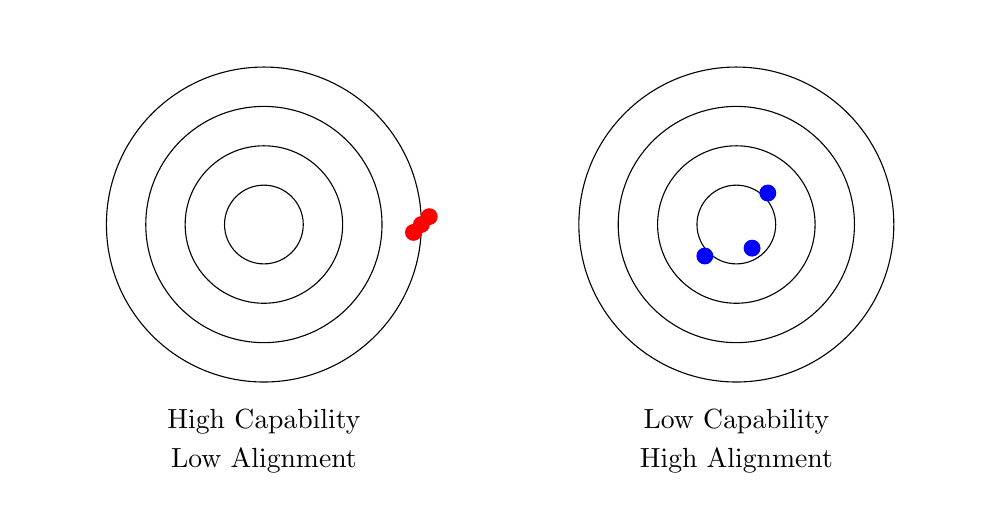
\begin{tikzpicture}
    % white background
    \begin{scope}[on background layer]
        \fill [white] (-3,-3.5) rectangle (9,2.5);
    \end{scope}

    % draw circles
    \draw[black] (0,0) circle (2cm);
    \draw[black] (0,0) circle (1.5cm);
    \draw[black] (0,0) circle (1cm);
    \draw[black] (0,0) circle (0.5cm);
    \draw[black] (6,0) circle (2cm);
    \draw[black] (6,0) circle (1.5cm);
    \draw[black] (6,0) circle (1cm);
    \draw[black] (6,0) circle (0.5cm);

    % draw points
    \draw[red, fill=red] (1.9,-0.1) circle (0.1cm);
    \draw[red, fill=red] (2.0,0.0) circle (0.1cm);
    \draw[red, fill=red] (2.1,0.1) circle (0.1cm);
    \draw[blue, fill=blue] (5.6,-0.4) circle (0.1cm);
    \draw[blue, fill=blue] (6.2,-0.3) circle (0.1cm);
    \draw[blue, fill=blue] (6.4,0.4) circle (0.1cm);

    % add labels
    \node at (0,-2.5) {High Capability};
    \node at (0,-3.0) {Low Alignment};
    \node at (6,-2.5) {Low Capability};
    \node at (6,-3.0) {High Alignment};

\end{tikzpicture}

\end{document}
